\documentclass[a4paper,10pt]{report}

\usepackage{packages/rapportutc}
%\usepackage{packages/include-packages}


%%%%%%%% Références %%%%%%%%
\usepackage{cleveref}
\usepackage{hyperref}
\usepackage[nottoc, notlof, notlot]{tocbibind} % bibliographie http://tex.stackexchange.com/questions/71129/bibliography-in-table-of-contents
\usepackage{natbib} % bibliographie

%%%%%%%% Code informatique %%%%%%%%
\usepackage{packages/Sweave} %package d'affichage des codes R
\usepackage{listings} % pour hightlight code

%%%%%%%% Formules mathématiques %%%%%%%%
\usepackage{amsmath, amsthm, amssymb, graphics, setspace} %packages de mathématiques
\usepackage{chemist} %formule chimique 

%%%%%%%% Mise en forme %%%%%%%%
% Mise en forme graphique
\usepackage{graphicx,wrapfig,lipsum} % pour afficher des figures à côté du texte
\usepackage[linewidth=1pt]{mdframed} % permet de générer et gérer des frames
\usepackage{rotating} % rotations on tables, captions, text, ...
% Mise en forme images et tableaux
\usepackage{float} % permet de spécifier l'option "H" aux captions afin de les positionner de manière fixe
\usepackage{subcaption} % permet d'afficher plusieurs images dans une caption
\usepackage{array} % meilleurs "table" et "tabular"
% Mise en forme texte
\usepackage{setspace} % permet de spécifier l'espacement interligne
\usepackage{ulem} % \sout{Texte à barrer} \xout{Texte à hachurer} \uwave{Texte à souligner par une vaguelette}
\usepackage{calc,enumitem}  % Mise en forme l'environnement itemsize description etc.
\usepackage{color} % utilisation de couleurs
\usepackage{ae,aecompl} % Vir­tual fonts for T1 en­coded CMR-fonts
\usepackage{pifont} % com­mands for Pi fonts (Ding­bats, Sym­bol, etc.)
\usepackage{comment} % Selectively include/exclude portions of text \comment....\endcomment

\onehalfspacing % espacement interligne
\setlength{\parindent}{.5em} % indentation des retraits de première ligne

%%%%%%%%%%%%%%%%%%%%%%%%%%%%%%%%%%%%%%%%%%%%%%%%%%%%%%%%%%%%%%%%%%%%%%%%%%%% 

\title{TP 2 - Classification automatique}
\author{LU Han - HAMONNAIS Raphaël}
\date{\today}

\uv{SY09}
\branche{Génie Informatique}
\filiere{Fouille de Données et Décisionnel}
%%%%%%%%%%%%%%%%%%%%%%%%%%%%%%%%%%%%%%%%%%%%%%%%%%%%%%%%%%%%%%%%%%%%%%%%%%%%

\begin{document}

\renewcommand{\labelitemi}{\large\textcolor{tatoebagreen}{\fg}}
\newgeometry{top=2.5cm,bottom=2cm,left=2cm,right=2cm}
\groovypdtitre
\restoregeometry % restaure la géométrie par défaut de latex

%%%%%%%%%%%%%%%%%%%%%%%%%%%%%%%%%%%%%%%%%%%%%%%%%%%%%%%%%%%%%%%%%%%%%%%%%%%% 

\tableofcontents

%%%%%%%%%%%%%%%%%%%%%%%%%%%%%%%%%%%%%%%%%%%%%%%%%%%%%%%%%%%%%%%%%%%%%%%%%%%%



\chapter{Visualisation des données}

\section{Visualisation des données Iris}

\begin{figure}[H]
	\centering
	\captionsetup{justification=centering, margin=2cm}
	\begin{subfigure}[b]{0.5\linewidth}
		\centering
		\captionsetup{justification=centering, margin=1cm}
		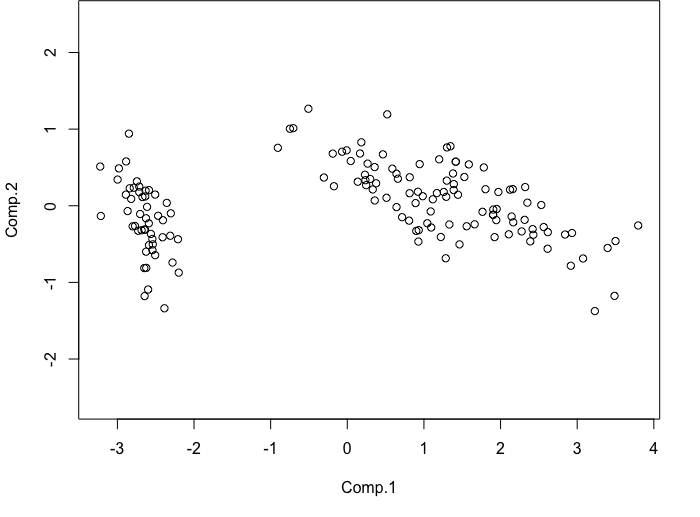
\includegraphics[width=1\linewidth]{img/1-iris-acp-premier-plan-factoriel}
		\caption{\small Données \texttt{Iris} dans le premier plan factoriel sans tenir compte de l'espèce}
		\label{fig:1-iris-acp-premier-plan-factoriel}
	\end{subfigure}%
	\begin{subfigure}[b]{0.5\linewidth}
		\centering
		\captionsetup{justification=centering, margin=1cm}
		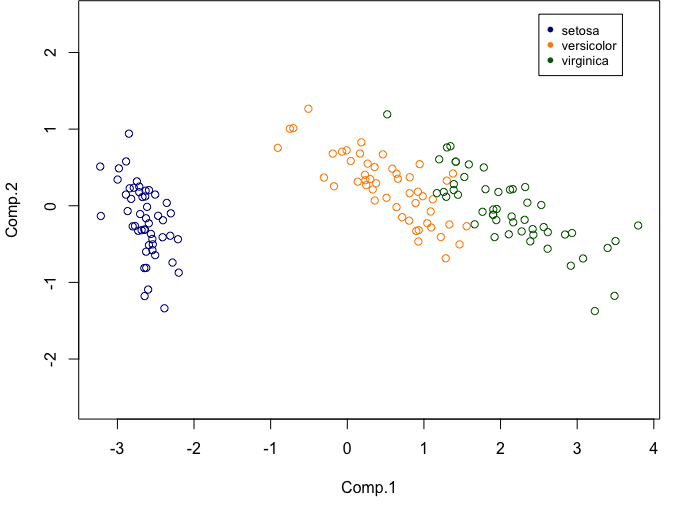
\includegraphics[width=1\linewidth]{img/1-iris-acp-premier-plan-factoriel-discr-species}
		\caption{\small Données \texttt{Iris} dans le premier plan factoriel en tenant compte de l'espèce}
		\label{fig:1-iris-acp-premier-plan-factoriel-discr-species}
	\end{subfigure}%
	\caption{\small Représentation des données \texttt{Iris} dans le premier plan factoriel après ACP}
	\label{fig:1-iris-acp-representation-graphique}%
\end{figure}

\begin{itemize}
	\item Affichage dans le premier plan factoriel sans tenir compte de l'espèce
	\begin{itemize}
		\item On observe deux groupes bien distincts (voir \autoref{fig:1-iris-acp-premier-plan-factoriel}).
	\end{itemize}

	\item Affichage dans le premier plan factoriel en tenant compte de l'espèce
	\begin{itemize}
		\item On voit qu'un des deux groupes précédemment observé est en fait constitué de deux espèces différentes (voir \autoref{fig:1-iris-acp-premier-plan-factoriel-discr-species})~;
		\item On obtient donc deux informations précieuses~:
		\begin{itemize}
			\item Les méthodes de classification géométriques tendront à nous donner deux classes ;
			\item On sait que les données contiennent en réalité trois classes bien distinctes quand le facteur discriminant est l'espèce ;
			\item Il faudra donc faire attention à ce qu'on cherche à obtenir~: une nouvelle classification en X classes sans tenir compte de l'espèce, et auquel cas on obtiendra surement deux classes. Ou bien une classification en fonction de l'espèce et alors il faudra spécifier qu'on cherche à obtenir trois classes.
		\end{itemize}
	\end{itemize}
\end{itemize}





\section{Visualisation des données Crabs}

\begin{figure}[H]
	\centering
	\captionsetup{justification=centering, margin=2cm}
	\begin{subfigure}[b]{0.5\linewidth}
		\centering
		\captionsetup{justification=centering, margin=1cm}
		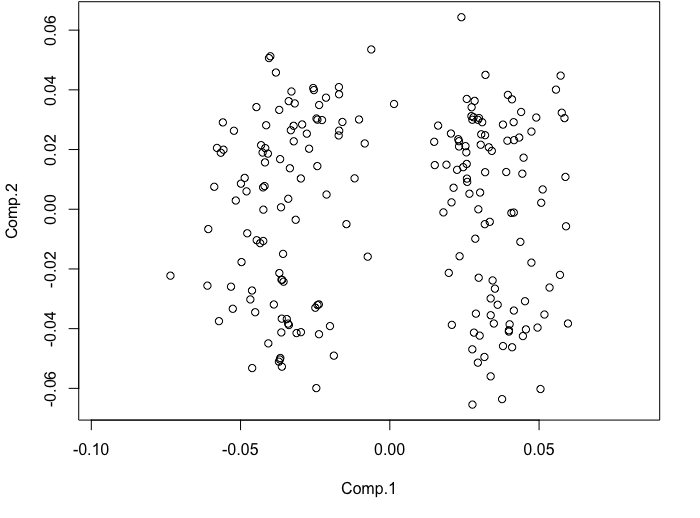
\includegraphics[width=1\linewidth]{img/1-crabs-acp-premier-plan-factoriel}
		\caption{\small Données \texttt{Crabs} dans le premier plan factoriel sans tenir compte de l'espèce ou du sexe}
		\label{fig:1-crabs-acp-premier-plan-factoriel}
	\end{subfigure}%
	\begin{subfigure}[b]{0.5\linewidth}
		\centering
		\captionsetup{justification=centering, margin=1cm}
		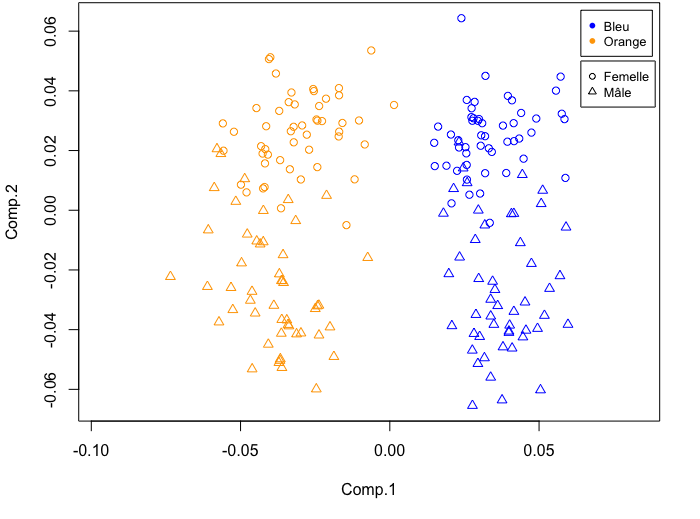
\includegraphics[width=1\linewidth]{img/1-crabs-acp-premier-plan-factoriel-discr-species-and-sex}
		\caption{\small Données \texttt{Crabs} dans le premier plan factoriel en tenant compte de l'espèce et du sexe}
		\label{fig:1-crabs-acp-premier-plan-factoriel-discr-species-and-sex}
	\end{subfigure}%
	\caption{\small Représentation des données \texttt{Crabs} dans le premier plan factoriel après ACP}
	\label{fig:1-crabs-acp-representation-graphique}%
\end{figure}


\begin{itemize}
	\item Affichage dans le premier plan factoriel sans tenir compte de l'espèce ou du sexe
	\begin{itemize}
		\item On observe deux groupes bien distincts (voir \autoref{fig:1-crabs-acp-premier-plan-factoriel}).
	\end{itemize}
	
	\item Affichage dans le premier plan factoriel en tenant compte de l'espèce et du sexe (voir \autoref{fig:1-crabs-acp-premier-plan-factoriel-discr-species-and-sex})
	\begin{itemize}
		\item On constate que les deux groupes observés précédemment correspondent à l'espèce des crabes ;
		\item On voit aussi apparaître deux autres groupes au sein des premiers qui délimitent le sexe ;
		\item On va donc chercher à faire une classification à 4 classes ;
		\item On note quand même que la délimitation entre les sexes est plus floue que celle entre les espèces.
	\end{itemize}
\end{itemize}



\section{Visualisation des données Mutation}

Les données \texttt{Mutation} représentent par le biais d'une matrice de dissimilarités les liens entre espèces~: plus la distance (dissimilarité) est faible, plus les espèces sont proches.

Nous allons effectuer une Analyse Factorielle de Tableau de Distance (AFTD). On rappelle que l’AFTD peut être vue comme un équivalent de l’ACP pour des données se présentant sous la forme d’un tableau $n \times n$ de dissimilarités $\delta_{ij}$ entre $n$ individus ($i,\ j \in \{1,...,n\}$)~: elle calcule une représentation multidimensionnelle de ces individus (dont le tableau de dissimilarités ne donne qu’une description implicite) dans un espace euclidien de dimension $p \leqslant n$. Cette représentation est exacte lorsque les dissimilarités sont des distances euclidiennes, ce qui n'est pas toujours le cas.
\\Après sélection d’un certain nombre de variables, la qualité de la représentation peut être évaluée numériquement par un critère similaire au pourcentage d’inertie de l’ACP, ou graphiquement au moyen d’un diagramme de Shepard : sur ce graphique, la distance $d_{ij} = d(x_i,x_j)$ entre les représentations de $x_i$ et $x_j$ déterminées par l’AFTD est représentée en fonction de la dissimilarité initiale $\delta_{ij}$, pour chaque couple d’individus $(x_i,x_j)$.


\subsection{Données Mutation dans le premier plan factoriel après AFTD}
\label{subsection:1-3-1-mut-premier-plan-factoriel}

\begin{figure}[H]
	\centering
	\captionsetup{justification=centering, margin=4cm}
	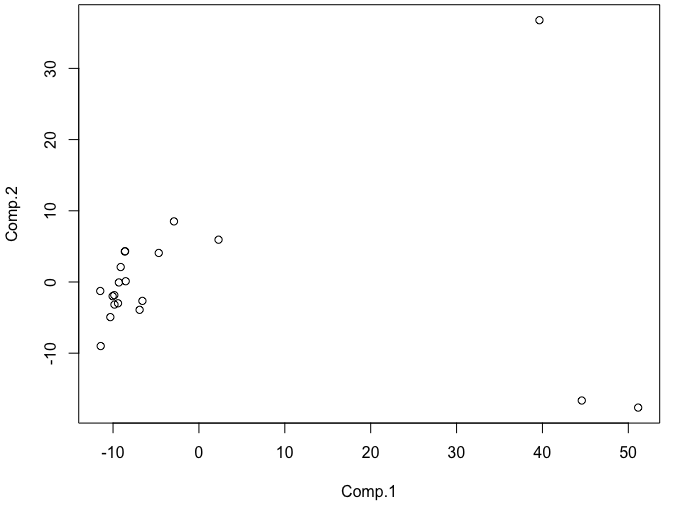
\includegraphics[width=.5\linewidth]{img/1-mut-acp-aftd-premier-plan-factoriel}
	\caption{\small Représentation euclidienne des données \texttt{Mutation} en deux dimensions par AFTD}	
	\label{fig:1-mut-acp-aftd-deux-dimensions}%
\end{figure}


Cette représentation a le mérite de nous permettre d'appréhender plus facilement le tableau de dissimilarités~: on voit clairement que beaucoup des espèces sont proches les unes des autres. Certaines très proches. On voit aussi que trois d'entre elles sont particulièrement éloignées.

On pourrait former deux classes~: la première regroupant l'ensemble des points proches, et la seconde les trois points éloignés. Ou bien trois, si on décide que l'espèce tout en haut à droite du graphique est trop loin pour être intégrée à une classe. Il est aussi tout à fait possible de subdiviser la première classe d'espèces proches les unes des autres en plusieurs classes plus petites.




\subsection{Analyse de la qualité de la représentation par AFTD}

Certaines des valeurs propres (inertie expliquée de la composante principale correspondante) sont négatives. Calculer le pourcentage d'inertie expliquée demande alors de faire un choix~: transformer les valeurs propres négatives en leur inverse positif (valeur absolue) ou bien ne tenir compte que des valeurs propres positives. Nous avons ici effectué les calculs avec les deux possibilité afin de comparer les résultats (voir \autoref{table:1-mut-acp-aftd-inertie-valeurs-absolues} et \autoref{table:1-mut-acp-aftd-inertie-valeurs-positives}).

\begin{table}[H]
	\centering
	\begin{tabular}{r|rrrrr}
		& Comp.1 & Comp.2 & Comp.3 & Comp.4 & Comp.5 \\ 
		\hline
		\small Pourcentage d'inertie expliquée & 52.71 & 16.01 & 10.94 & 6.72 & 4.78 \\ 
		\small Pourcentage cumulé d'inertie expliquée & 52.71 & 68.72 & 79.67 & 86.38 & 91.16 \\ 
	\end{tabular}
	\caption{Inertie avec valeurs absolues}
	\label{table:1-mut-acp-aftd-inertie-valeurs-absolues}
\end{table}

\begin{table}[H]
	\centering
	\begin{tabular}{r|rrrrr}
		& Comp.1 & Comp.2 & Comp.3 & Comp.4 & Comp.5 \\ 
		\hline
		\small Pourcentage d'inertie expliquée & 53.43 & 16.23 & 11.09 & 6.81 & 4.84 \\ 
		\small Pourcentage cumulé d'inertie expliquée & 53.43 & 69.66 & 80.75 & 87.56 & 92.40 \\ 
	\end{tabular}
	\caption{Inertie avec valeurs positives seulement}
	\label{table:1-mut-acp-aftd-inertie-valeurs-positives}
\end{table}

On remarque que les pourcentages d'inertie expliquée ne varient pas énormément entre les deux choix de calcul. Cela s'explique par la faible importance des valeurs propres négatives dans ce jeu de données.

Pour ce qui est de la qualité de la représentation, on voit très vite qu'avec simplement deux dimensions, on n'obtient qu'environ 69\% d'inertie expliquée. C'est relativement peu pour une ACP, mais cela peut être suffisant pour une représentation simple des données. Tenir compte de trois, quatre ou cinq dimensions nous permet à chaque fois de mieux représenter des données, avec respectivement 80\%, 87\% et 92\% d'inertie cumulée.\\

On remarque aussi cette augmentation de qualité de représentation des données initiales lorsqu'on regarde les diagrammes de Shepard~:

\begin{figure}[H]
	\centering
	\captionsetup{justification=centering, margin=3cm}
	\begin{subfigure}[b]{0.25\linewidth}
		\centering
		\captionsetup{justification=centering}
		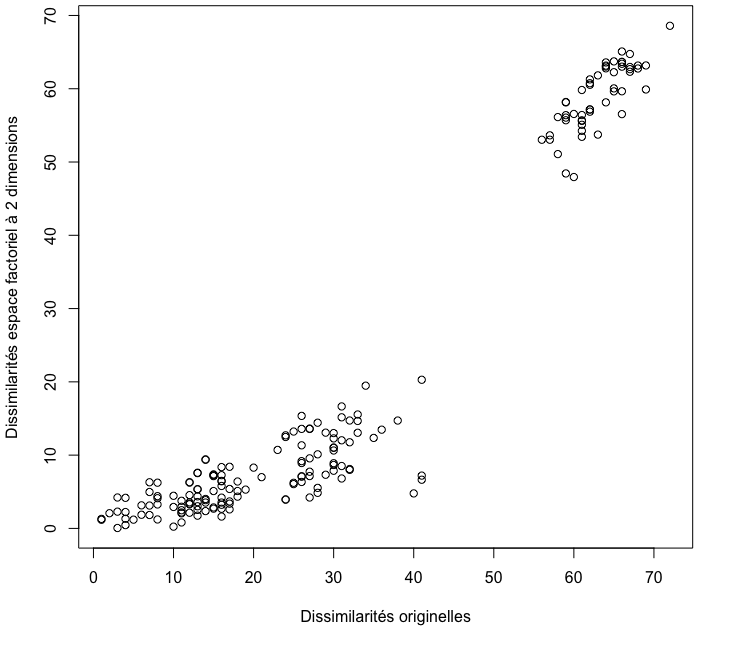
\includegraphics[width=1\linewidth]{img/1-mut-acp-aftd-diag-shepard-2-dim}
		\caption{\small Diagramme de Shepard\\(2 dimensions)}
		\label{fig:1-mut-acp-aftd-diag-shepard-2-dim}
	\end{subfigure}%
	\begin{subfigure}[b]{0.25\linewidth}
		\centering
		\captionsetup{justification=centering}
		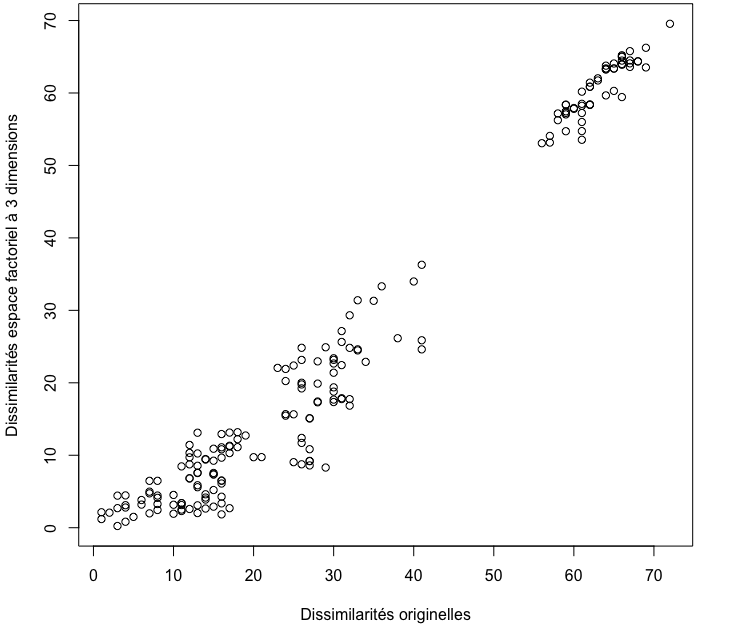
\includegraphics[width=1\linewidth]{img/1-mut-acp-aftd-diag-shepard-3-dim}
		\caption{\small Diagramme de Shepard\\(3 dimensions)}
		\label{fig:1-mut-acp-aftd-diag-shepard-3-dim}
	\end{subfigure}%
	\begin{subfigure}[b]{0.25\linewidth}
		\centering
		\captionsetup{justification=centering}
		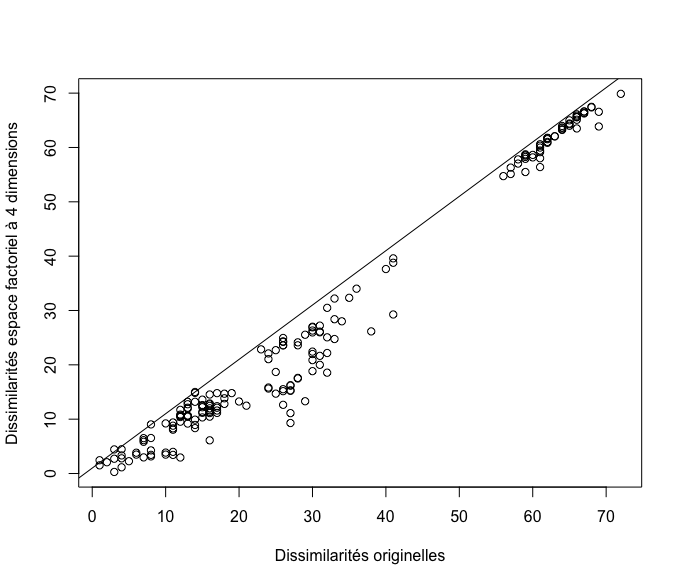
\includegraphics[width=1\linewidth]{img/1-mut-acp-aftd-diag-shepard-4-dim}
		\caption{\small Diagramme de Shepard\\(4 dimensions)}
		\label{fig:1-mut-acp-aftd-diag-shepard-4-dim}
	\end{subfigure}%
	\begin{subfigure}[b]{0.25\linewidth}
		\centering
		\captionsetup{justification=centering}
		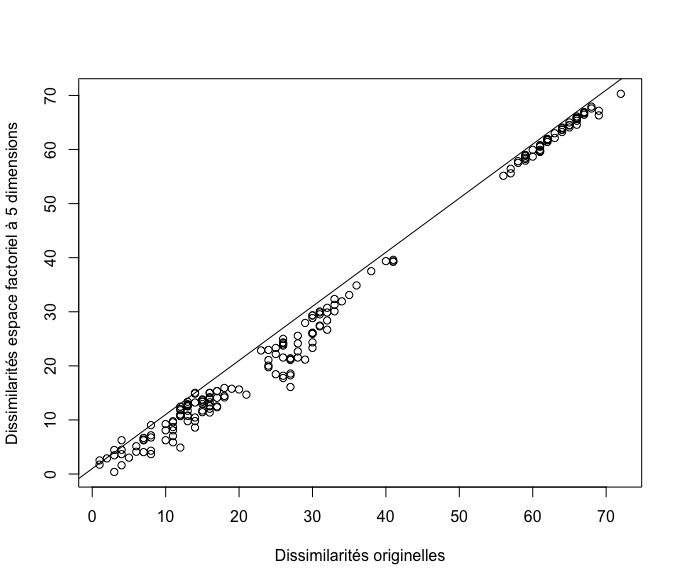
\includegraphics[width=1\linewidth]{img/1-mut-acp-aftd-diag-shepard-5-dim}
		\caption{\small Diagramme de Shepard\\(5 dimensions)}
		\label{fig:1-mut-acp-aftd-diag-shepard-5-dim}
	\end{subfigure}%
	\caption{\small Diagrammes de Shepard pour les dimensions 2 à 5}
	\label{fig:1-mut-acp-aftd-diag-shepard}%
\end{figure}

L'axe des abscisses représente les dissimilarités originelles avant AFTD et l'axe des ordonnées les distances euclidiennes entre les observations sur le nouvel espace factoriel obtenu par l'AFTD.

Plus le nombre de dimensions augmente, plus les valeurs des dissimilarités avant et après AFTD s'approchent de la droite $y = x$, c'est à dire une dissimilarité initiale égale à la distance entre les individus représentés dans l'espace euclidien à $k$ dimensions défini par l'AFTD.







\chapter{Classification hiérarchique}

\section{Classification hiérarchique ascendante sur les données Mutation}
\label{section:mut-class-hierarchique}

\textit{Remarque~: certains critères d'agrégation sont "pondérés". Cela signifie que les classes sont considérées comme étant de poids équivalents, quel que soit leur effectif.}

\begin{figure}[H]
	\centering
	\captionsetup{justification=centering, margin=3cm}
	\begin{subfigure}[b]{0.4\linewidth}
		\centering
		\captionsetup{justification=centering}
		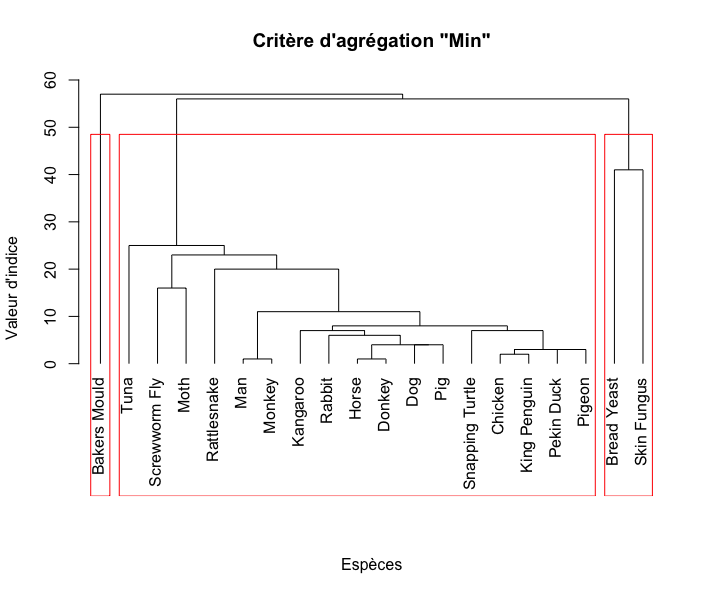
\includegraphics[width=1\linewidth]{img/2-1-mut-hierarchie-min}
		\caption{\small Critère agrégation Min}
		\label{fig:2-1-mut-hierarchie-min}
	\end{subfigure}%
	\begin{subfigure}[b]{0.4\linewidth}
		\centering
		\captionsetup{justification=centering}
		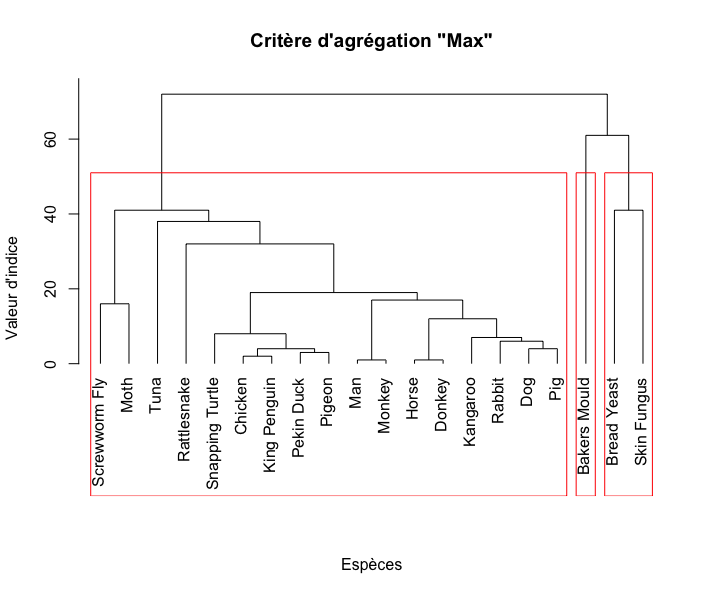
\includegraphics[width=1\linewidth]{img/2-1-mut-hierarchie-max}
		\caption{\small Critère agrégation Max}
		\label{fig:2-1-mut-hierarchie-max}
	\end{subfigure}%
	\caption{\small Classification avec les critères d'agrégation Min et Max}
	\label{fig:2-1-classification-mut-min-max}%
\end{figure}

\begin{figure}[H]
	\centering
	\captionsetup{justification=centering, margin=3cm}
	\begin{subfigure}[b]{0.4\linewidth}
		\centering
		\captionsetup{justification=centering}
		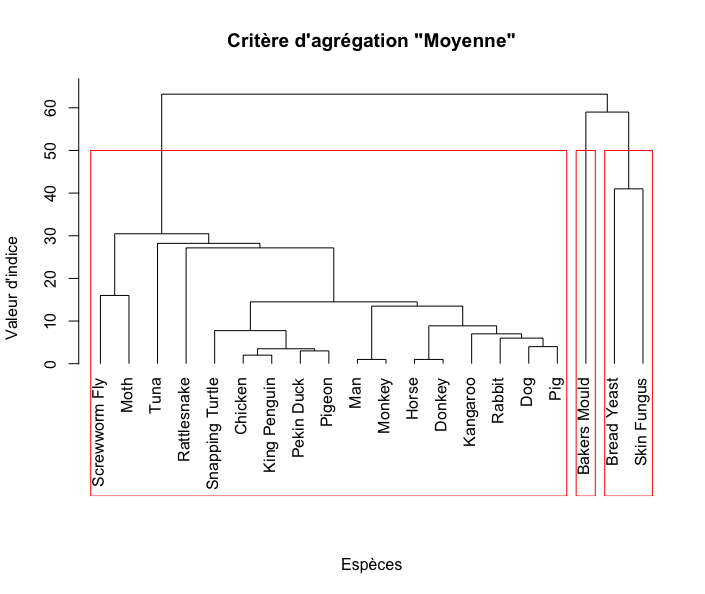
\includegraphics[width=1\linewidth]{img/2-1-mut-hierarchie-moy}
		\caption{\small Critère agrégation Moyenne}
		\label{fig:2-1-mut-hierarchie-moy}
	\end{subfigure}%
	\begin{subfigure}[b]{0.4\linewidth}
		\centering
		\captionsetup{justification=centering}
		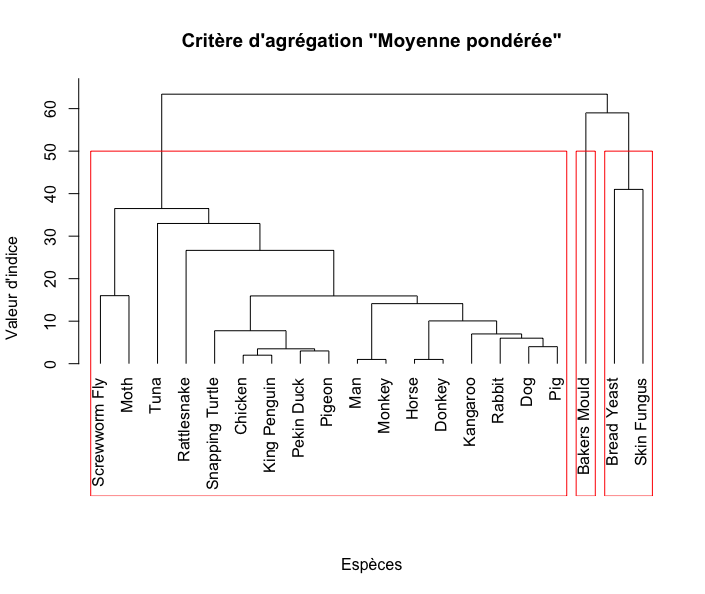
\includegraphics[width=1\linewidth]{img/2-1-mut-hierarchie-moy-ponderee}
		\caption{\small Critère agrégation Moyenne pondérée}
		\label{fig:2-1-mut-hierarchie-moy-ponderee}
	\end{subfigure}%
	\caption{\small Classification avec les critères d'agrégation Moyenne et Moyenne pondérée}
	\label{fig:2-1-classification-mut-moy}%
\end{figure}


\begin{figure}[H]
	\centering
	\captionsetup{justification=centering, margin=3cm}
	\begin{subfigure}[b]{0.4\linewidth}
		\centering
		\captionsetup{justification=centering}
		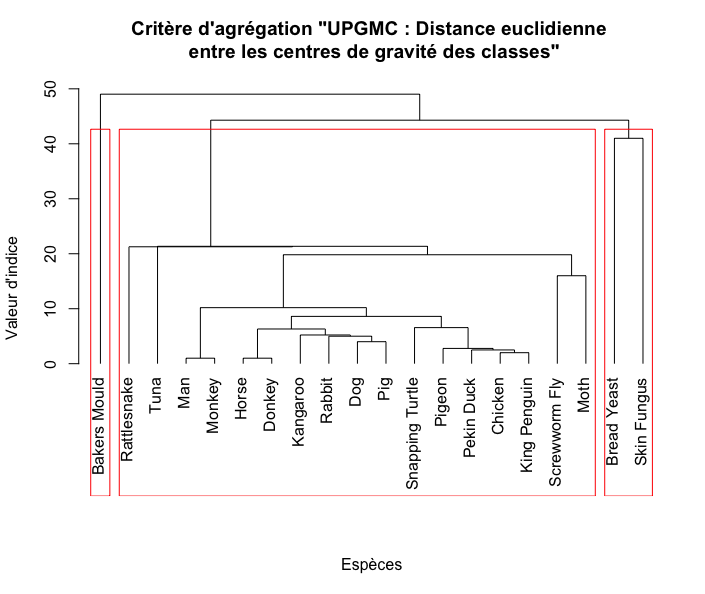
\includegraphics[width=1\linewidth]{img/2-1-mut-hierarchie-centroid}
		\caption{\small Critère agrégation distance inter-classe}
		\label{fig:2-1-mut-hierarchie-centroid}
	\end{subfigure}%
	\begin{subfigure}[b]{0.4\linewidth}
		\centering
		\captionsetup{justification=centering}
		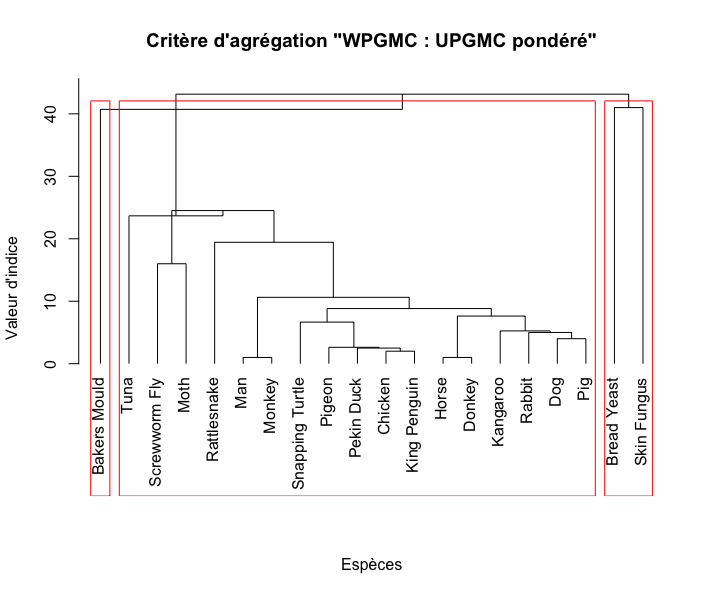
\includegraphics[width=1\linewidth]{img/2-1-mut-hierarchie-centroid-ponderee}
		\caption{\small Critère agrégation distance inter-classe pondérée}
		\label{fig:2-1-mut-hierarchie-centroid-ponderee}
	\end{subfigure}%
	\caption{\small Classification avec les critères d'agrégation de distance inter-classe (distance entre centres de gravité des classes)}
	\label{fig:2-1-classification-mut-centroid}%
\end{figure}


\begin{figure}[H]
	\centering
	\captionsetup{justification=centering, margin=3cm}
	\begin{subfigure}[b]{0.4\linewidth}
		\centering
		\captionsetup{justification=centering}
		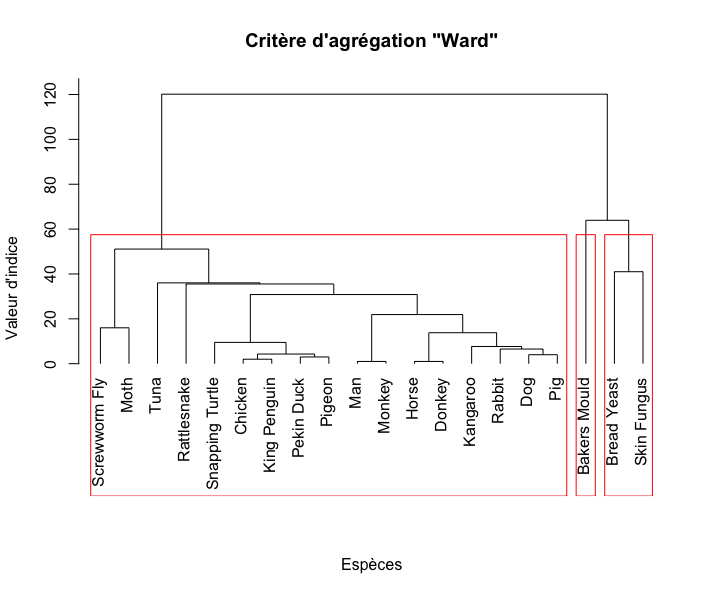
\includegraphics[width=1\linewidth]{img/2-1-mut-hierarchie-ward}
		%\caption{\small Critère agrégation Ward}
		\label{fig:2-1-mut-hierarchie-ward}
	\end{subfigure}%
	\caption{\small Classification avec le critère d'agrégation de Ward}
	\label{fig:2-1-classification-mut-ward}%
\end{figure}



La première chose qu'on remarque est que, lorsqu'on divise en trois classes tel que nous le suggérait la représentation graphique des données après AFTD (cf. \autoref{subsection:1-3-1-mut-premier-plan-factoriel}), tous les critères d'agrégation donnent les mêmes classes. A savoir \textit{\{Bakers Mould\}}, \textit{\{Bread Yeast, Skin Fungus\}}, et le reste dans la dernière classe.

Il est aussi intéressant de remarquer que deux des critères d'agrégation ne sont pas monotones (cf. \autoref{fig:2-1-mut-hierarchie-centroid} et \autoref{fig:2-1-mut-hierarchie-centroid-ponderee}). On voit en effet que l'indice n'est pas décroissant.



\section{Classification hiérarchique sur les données Iris}



\subsection{Classification hiérarchique ascendante}

\begin{figure}[H]
	\centering
	\captionsetup{justification=centering, margin=3cm}
	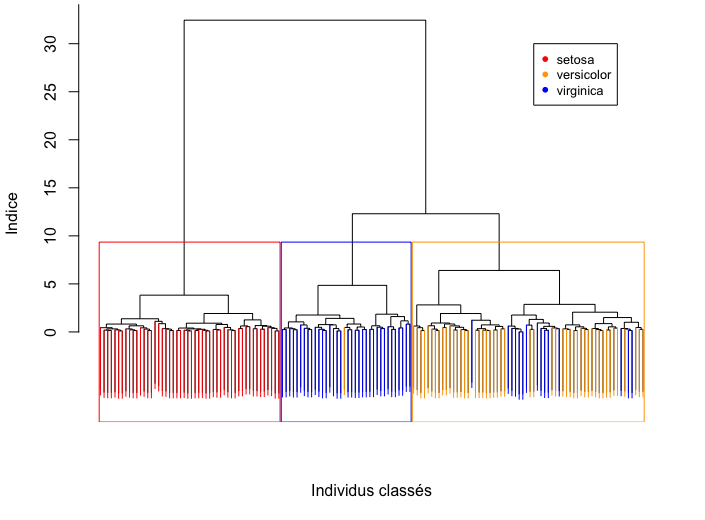
\includegraphics[width=.6\linewidth]{img/2-2-1-iris-class-hierarchique-asc}
	\caption{Iris : classification hiérarchique ascendante}
	\label{2-2-1-iris-class-hierarchique-asc}%
\end{figure}

La classification identifie très bien les individus de l'espèce \textit{setosa}. Par contre, elle tend à confondre certains individus des espèces \textit{versicolor} et \textit{virginica}. Compte tenu de la représentation graphique obtenue après ACP (cf. \autoref{fig:1-iris-acp-premier-plan-factoriel-discr-species}), ce n'est pas étonnant, ces deux espèces étant très proches sur le graphe, contrairement à \textit{setosa} qui est bien distincte graphiquement parlant.


\subsection{Classification hiérarchique descendante}

\begin{figure}[H]
	\centering
	\captionsetup{justification=centering, margin=3cm}
	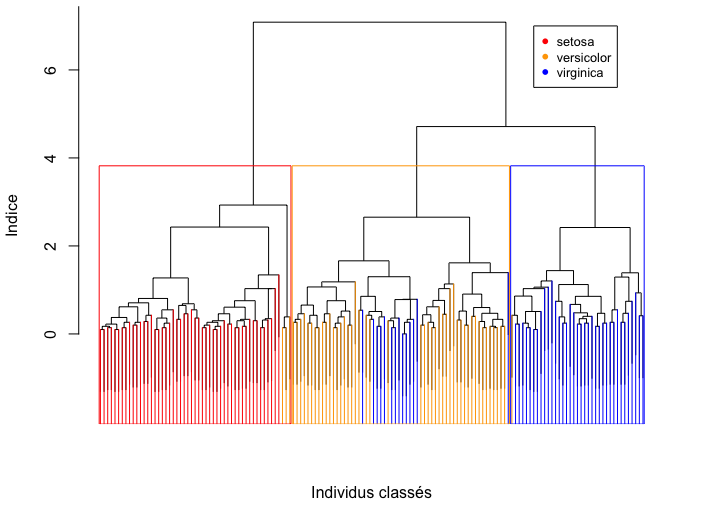
\includegraphics[width=.6\linewidth]{img/2-2-1-iris-class-hierarchique-desc}
	\caption{Iris : classification hiérarchique descendante}
	\label{2-2-1-iris-class-hierarchique-desc}%
\end{figure}


La classification hiérarchique descendante confond elle aussi certains des individus des espèces \textit{versicolor} et \textit{virginica}. Mais elle classe en plus certains individus de l'espèce \textit{versicolor} dans la classe contenant les individus d'espèce \textit{setosa}. Elle semble à priori moins précise que la classification hiérarchique ascendante.\\

Afin de savoir laquelle des deux méthodes reste la plus précise, nous utilisons l'indice de Rand corrigé. Le principe est de sélectionner l'ensemble des paires possibles d'individus au sein de chaque partition et comparer leur classement au classement initial qui est connu. La valeur de cet indice est comprise entre 0 et 1~: plus elle se rapproche de 1, plus la classification obtenue est proche de la classification initiale.\\

Valeurs obtenues~:
\begin{itemize}
	\item Classification ascendante~: 0.73
	\item Classification descendante~: 0.69
\end{itemize}

On en déduit que la classification ascendante est meilleure pour ce jeu de données, bien que de peu.




\chapter{Méthode des centres mobiles (K-Means)}



\section{Données Iris}


\subsection{Partition en $K \in {2,3,4}$}


\begin{figure}[H]
	\centering
	\captionsetup{justification=centering, margin=3cm}
	\begin{subfigure}[b]{0.33\linewidth}
		\centering
		\captionsetup{justification=centering}
		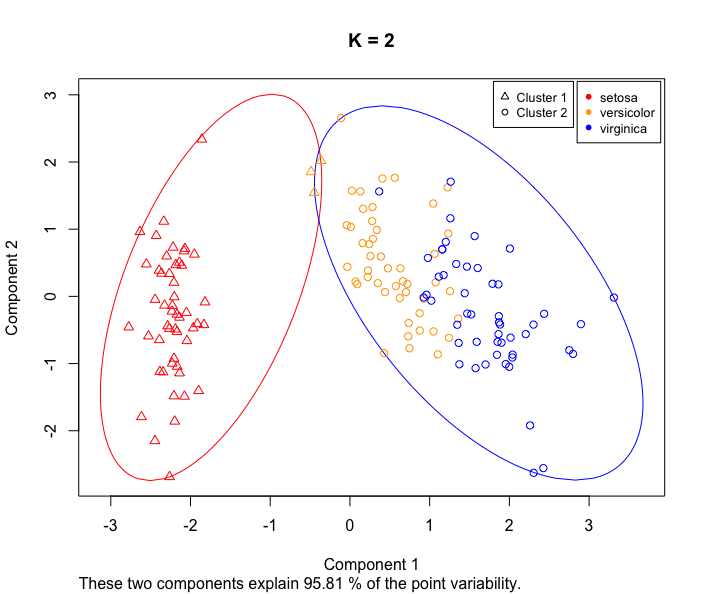
\includegraphics[width=1\linewidth]{img/3-1-1-iris-kmeans-2}
		\caption{\small Centres mobiles avec K = 2}
		\label{fig:3-1-1-iris-kmeans-2}
	\end{subfigure}%
	\begin{subfigure}[b]{0.33\linewidth}
		\centering
		\captionsetup{justification=centering}
		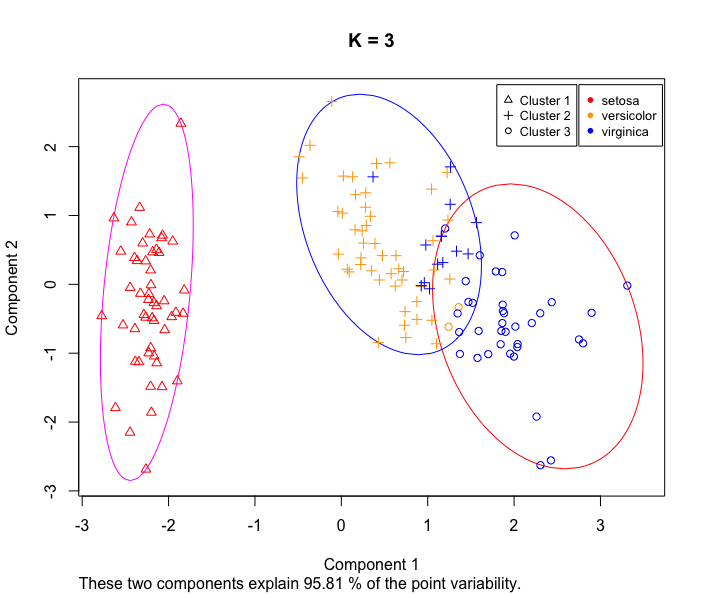
\includegraphics[width=1\linewidth]{img/3-1-1-iris-kmeans-3}
		\caption{\small Centres mobiles avec K = 3}
		\label{fig:3-1-1-iris-kmeans-3}
	\end{subfigure}%
	\begin{subfigure}[b]{0.33\linewidth}
		\centering
		\captionsetup{justification=centering}
		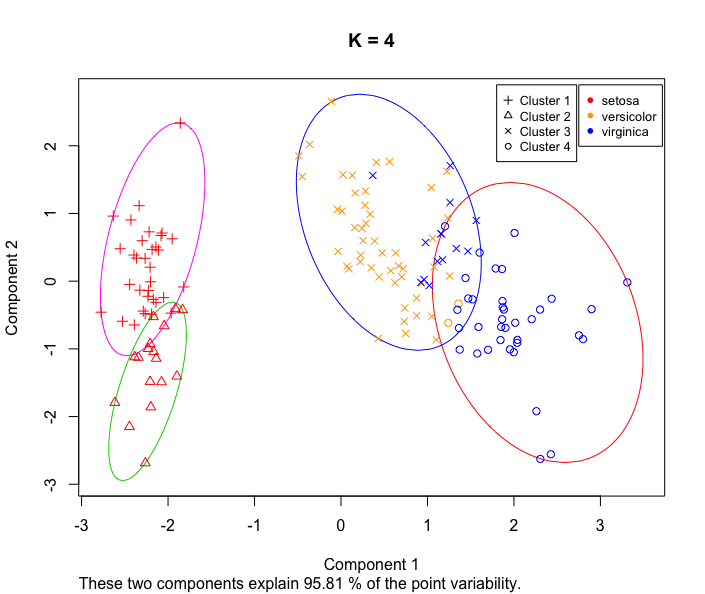
\includegraphics[width=1\linewidth]{img/3-1-1-iris-kmeans-4}
		\caption{\small Centres mobiles avec K = 4}
		\label{fig:3-1-1-iris-kmeans-4}
	\end{subfigure}%
	\caption{\small Iris : classification à l'aide de l'algorithme des centres mobiles en 2, 3 et 4 classes}
	\label{fig:3-1-1-kmeans-iris-en-2-3-4-classes}%
\end{figure}

Classifications obtenues sans recherche d'un critère de sélection minimal~:
\begin{itemize}
	\item La séparation en deux classes détecte bien les deux groupements de points qui sont visibles (voir \autoref{fig:1-iris-acp-premier-plan-factoriel})~;
	\item La classification en trois classes semble elle aussi avoir du sens car elle identifie les trois différentes espèces (voir \autoref{fig:1-iris-acp-premier-plan-factoriel-discr-species})~;
	\item La classification en 4 classes quant à elle divise la première en deux sous-classes différentes.
\end{itemize}

\subsection{Étude de la stabilité du résultat}

Afin d'étudier la stabilité du résultat, nous avons effectué 100 classifications consécutives. On s'aperçoit que l'algorithme donne toujours les deux mêmes classifications, présentées dans les tableaux \autoref{table:3-1-2-Différentes-inerties-intra-classe-obtenues} et \autoref{table:3-1-2-Différentes-classifications-obtenues}

\begin{table}[H]
	\centering
	\captionsetup{justification=centering, margin=3cm}
	\begin{tabular}{r|r|r}
		& Inertie intra classe & Fréquence d'apparition \\ 
		\hline
		Classification n° 1 & 0.53 &  76\% \\ 
		Classification n° 2 & 0.95 &  24\% \\ 
	\end{tabular}
	\caption{\small Différentes inerties intra-classe obtenues}
	\label{table:3-1-2-Différentes-inerties-intra-classe-obtenues}
\end{table}


\begin{table}[H]
	\centering
	\captionsetup{justification=centering, margin=3cm}
	\begin{subtable}{.3\textwidth}
		\centering
		\begin{tabular}{r|rrr}
			& 1 & 2 & 3 \\ 
			\hline
			setosa &   0 &  50 &   0 \\ 
			versicolor &  48 &   0 &   2 \\ 
			virginica &  14 &   0 &  36 \\ 
		\end{tabular}
		\caption{\small Classification n° 1}
	\end{subtable}
	\begin{subtable}{.3\textwidth}
		\centering
		\begin{tabular}{r|rrr}
			& 1 & 2 & 3 \\ 
			\hline
			setosa &  33 &  17 &   0 \\ 
			versicolor &   0 &   4 &  46 \\ 
			virginica &   0 &   0 &  50 \\ 
		\end{tabular}
		\caption{\small Classification n° 2}
	\end{subtable}
	\caption{\small Différentes classifications en fonction de l'inertie intra-classe}
	\label{table:3-1-2-Différentes-classifications-obtenues}
\end{table}


La classification numéro 1 est la meilleure dans le sens où elle minimise la valeur de l'inertie intra-classe de la partition. On peut d'ailleurs s'en assurer en comparant les représentations graphiques des deux classifications obtenues (voir \autoref{fig:3-1-2-Representation-Differentes-classifications-obtenues})~:



\begin{figure}[H]
	\centering
	\captionsetup{justification=centering, margin=3cm}
	\begin{subfigure}[b]{0.5\linewidth}
		\centering
		\captionsetup{justification=centering}
		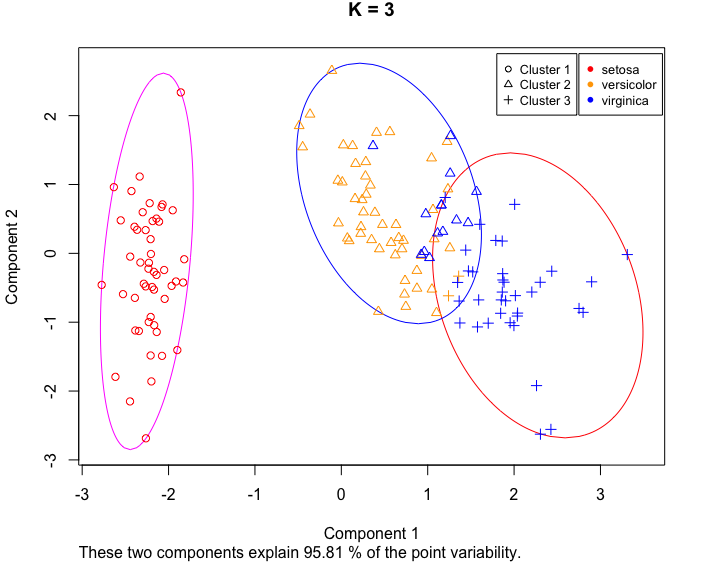
\includegraphics[width=1\linewidth]{img/3-1-2-iris-kmeans-3-min-inertie}
		\caption{\small Classification n°1}
		\label{fig:3-1-2-iris-kmeans-3-min-inertie}
	\end{subfigure}%
	\begin{subfigure}[b]{0.5\linewidth}
		\centering
		\captionsetup{justification=centering}
		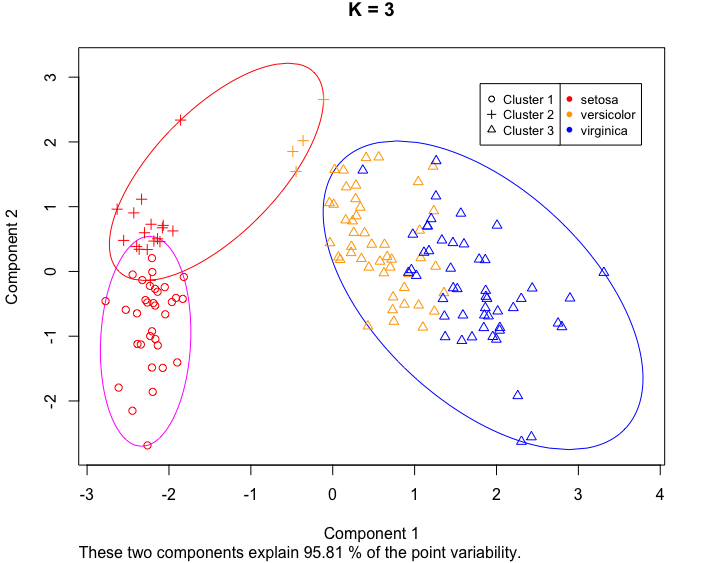
\includegraphics[width=1\linewidth]{img/3-1-2-iris-kmeans-3-max-inertie}
		\caption{\small Classification n°2}
		\label{fig:3-1-2-iris-kmeans-3-max-inertie}
	\end{subfigure}%
	\caption{\small Représentation des différentes classifications en fonction de l'inertie intra-classe}
	\label{fig:3-1-2-Representation-Differentes-classifications-obtenues}
\end{figure}

Même sans la connaissance préalable des données, la classification numéro deux semble bien moins pertinente que la première.


\subsection{Détermination du nombre de classes optimal}

La méthode du coude consiste à étudier la décroissance du critère (ici l'inertie intra-classe minimale) en fonction du nombre K de classes et choisir K avant le premier saut significatif.

\begin{figure}[H]
	\centering
	\captionsetup{justification=centering, margin=4cm}
	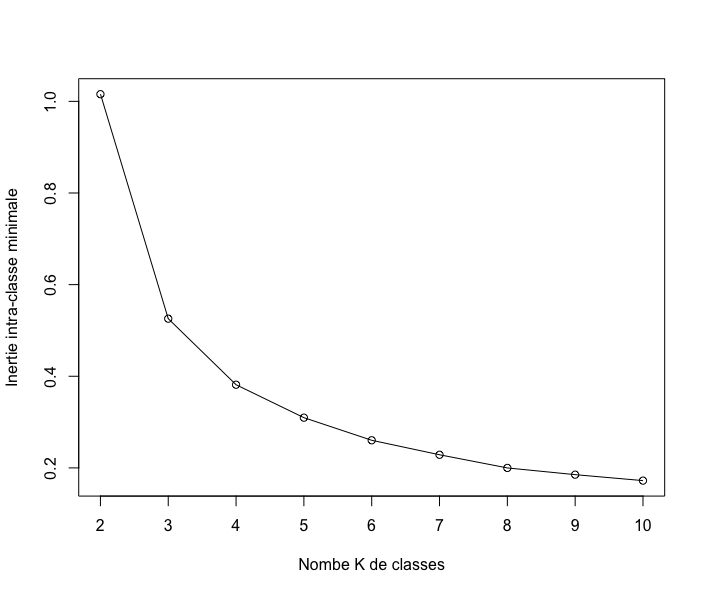
\includegraphics[width=.3\linewidth]{img/3-1-3-variation-inertie-minimale-en-fonction-de-K}
	\caption{\small Variation de l'inertie minimale en fonction du nombre K de classes}
	\label{fig:3-1-3-variation-inertie-minimale-en-fonction-de-K}
\end{figure}

D'après la courbe de variation, il est évident que le passage de 3 à 2 classes présente une augmentation importante du critère. Remarquons aussi que la pente de la droite entre les points K=3 et K=4 est plus importante que lorsque K est supérieur à 4.
On pourrait donc choisir 3 ou 4 comme étant le nombre optimal de classes, bien que 3 semble plus indiqué. La bonne solution est de tester avec les deux et de choisir ensuite en fonction des connaissances préalables des données que l'on a.

\subsection{Comparaison de la classification obtenue avec la classification connue des trois espèces}

\begin{figure}[H]
	\centering
	\captionsetup{justification=centering}
	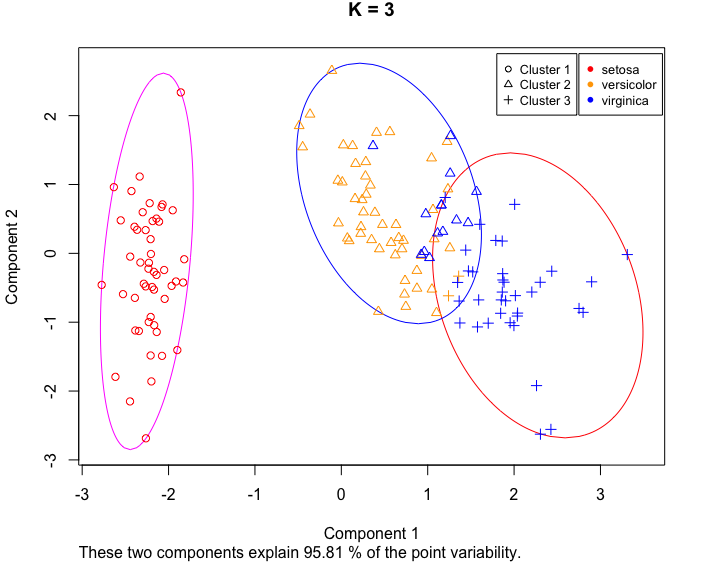
\includegraphics[width=.7\linewidth]{img/3-1-2-iris-kmeans-3-min-inertie}
	\caption{\small Comparaison de la classification K-Means avec la classification initiale connue}
	\label{fig:3-1-4-comparaison-classif-kmeans-vs-connue}
\end{figure}%

On remarque que la classification par les K-Means fait sens mais qu'elle commet quelques erreurs à jonction des espèces \textit{versicolor} et \textit{viginica}, comme le faisait la classification hiérarchique.





\section{Données Crabs}

\subsection{Classifications en 2 classes}

La classification en 2 classes n'est pas stable~:

\begin{table}[H]
	\centering
	\captionsetup{justification=centering, margin=3cm}
	\begin{tabular}{r|r|r}
		Classification n° & Inertie intra-classe & Pourcentage d'apparition \\
		\hline
		1 & 0.25878 & 73.80 \\ 
		2 & 0.35607 & 23.10 \\ 
		3 & 0.35754 & 1.00 \\ 
		4 & 0.358 & 1.20 \\ 
		5 & 0.3648 & 0.90 \\ 
	\end{tabular}
	\caption{Les 5 classifications obtenues sur 1000 essais}
	
\end{table}

Les deux premières classifications sont majoritaires. On remarquera que les classifications numéros 2 à 5 ont toutes une inertie intra-classe très proche les unes des autres~: ce sont des "variations" d'une même classification.

Lorsqu'on représente graphiquement ces classifications, on s'aperçoit qu'elles mettent en évidence une des catégories de l'individu~: son espèce (\autoref{fig:3-2-1-crabs-2-classes-classif-1-espece}) ou son sexe (\autoref{fig:3-2-1-crabs-2-classes-classif-2-sex}).

\begin{figure}[H]
	\centering
	\captionsetup{justification=centering, margin=1cm}
	\begin{subfigure}[b]{0.5\linewidth}
		\centering
		\captionsetup{justification=centering}
		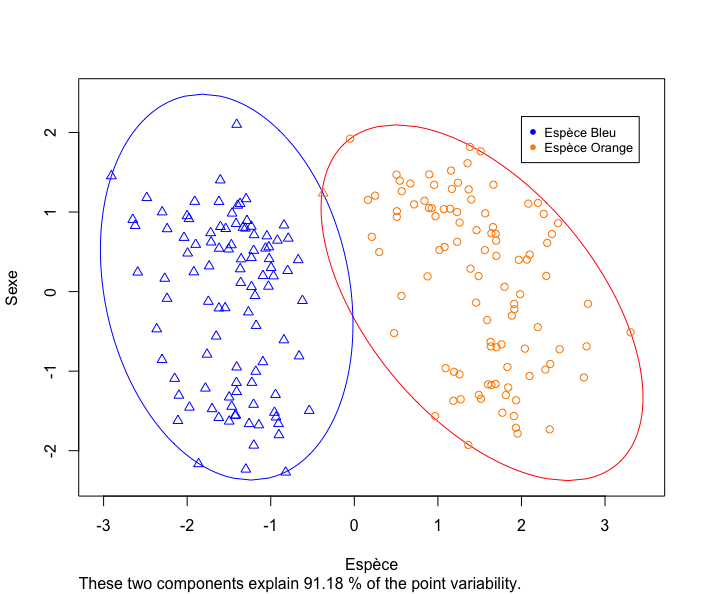
\includegraphics[width=1\linewidth]{img/3-2-1-crabs-2-classes-classif-1-espece}
		\caption{\small Classification n°1}
		\label{fig:3-2-1-crabs-2-classes-classif-1-espece}
	\end{subfigure}%
	\begin{subfigure}[b]{0.5\linewidth}
		\centering
		\captionsetup{justification=centering}
		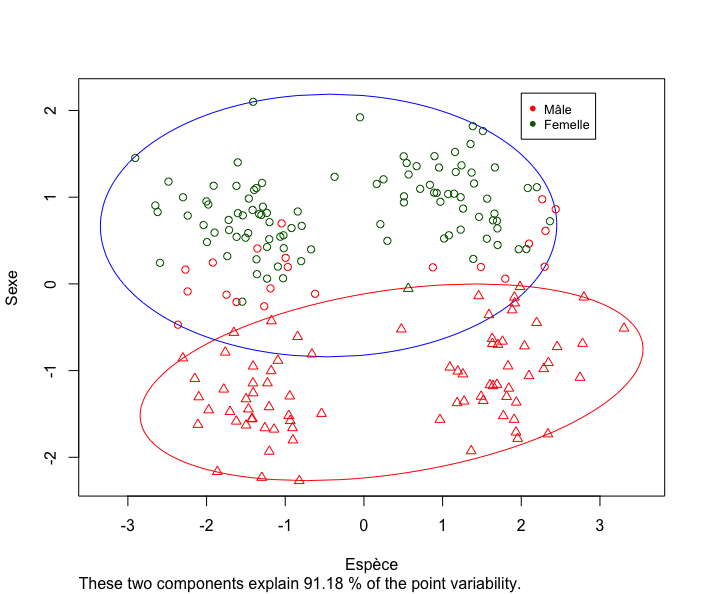
\includegraphics[width=1\linewidth]{img/3-2-1-crabs-2-classes-classif-2-sex}
		\caption{\small Classification n°2}
		\label{fig:3-2-1-crabs-2-classes-classif-2-sex}
	\end{subfigure}%
	\caption{\small Deux principales classifications des données \texttt{crabs} en deux classes}
	\label{fig:3-2-1-Crabs-kmeans-2-classes}
\end{figure}





\subsection{Classification en 4 classes}

On choisit la meilleure classification pour $K = 4$, c'est à dire celle qui minimise l'inertie intra-classe.


\begin{figure}[H]
	\centering
	\captionsetup{justification=centering, margin=2cm}
	\begin{subfigure}[b]{0.5\linewidth}
		\centering
		\captionsetup{justification=centering}
		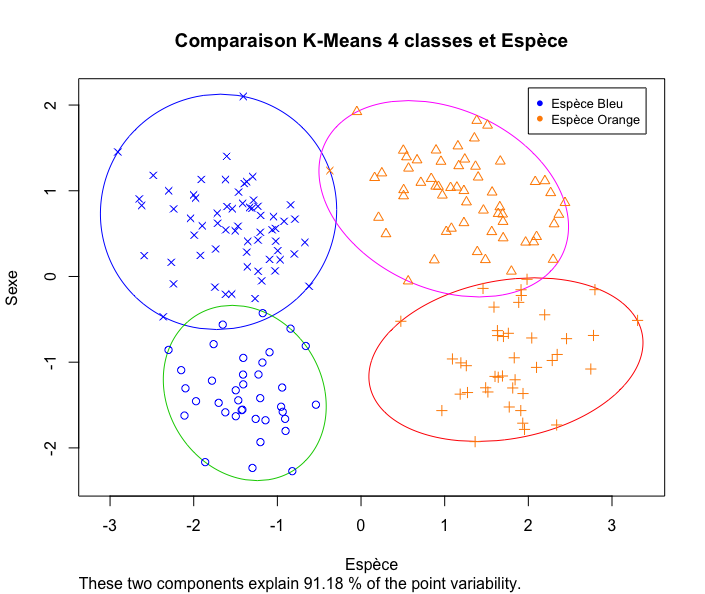
\includegraphics[width=1\linewidth]{img/3-2-2-crabs-kmeans-4-classes-espece}
		\caption{\small Comparaison avec l'espèce}
		\label{fig:3-2-2-crabs-kmeans-4-classes-espece}
	\end{subfigure}%
	\begin{subfigure}[b]{0.5\linewidth}
		\centering
		\captionsetup{justification=centering}
		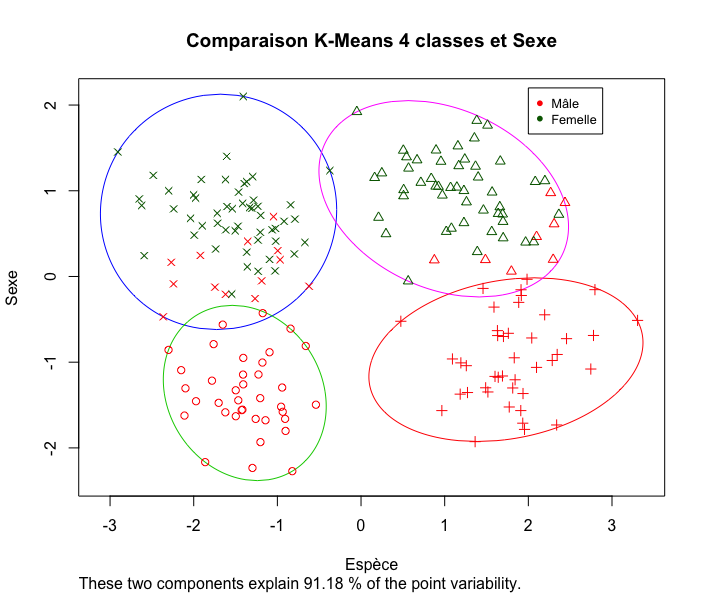
\includegraphics[width=1\linewidth]{img/3-2-2-crabs-kmeans-4-classes-sexe}
		\caption{\small Comparaison avec le sexe}
		\label{fig:3-2-2-crabs-kmeans-4-classes-sexe}
	\end{subfigure}%
	\caption{\small Comparaison entre la meilleure classification en 4 classes (obtenue via la méthode des centre mobiles) et les classes "Sexe" et "Espèce" connues}
	\label{fig:3-2-1-Crabs-kmeans-4-classes}
\end{figure}


On en conclut que la classification avec la méthode des centres mobiles est efficace~: elle identifie bien les 4 groupes différents d'individus en fonction de leur espèce et de leur sexe. Notons tout de même que la différenciation sur le critère de l'espèce est plus efficace que celle sur le critère du sexe~: seulement une erreur tandis qu'il y en a bien plus pour la différenciation du sexe des individus.




\section{Données Mutations}





La classification en 3 classes n'est pas stable~:

\begin{table}[H]
	\centering
	\captionsetup{justification=centering, margin=3cm}
	\begin{tabular}{r|r|r}
		Classification n° & Inertie intra-classe & Pourcentage d'apparition \\
		\hline
		1 & 181.092 & 30.90 \\ 
		2 & 219.91 & 18.00 \\ 
		3 & 245.904 & 24.60 \\ 
		4 & 248.75 & 11.30 \\ 
		5 & 254.623 & 8.80 \\ 
		6 & 261.861 & 6.40 \\ 
	\end{tabular}
	\caption{Classifications obtenues sur les données "Mutations" pour 1000 essais}
\end{table}



Voici la représentation graphique de chacune des six classifications possibles avec la méthode des K-means~:

\begin{figure}[H]
	\centering
	\captionsetup{justification=centering, margin=2cm}
	\begin{subfigure}[b]{0.5\linewidth}
		\centering
		\captionsetup{justification=centering}
		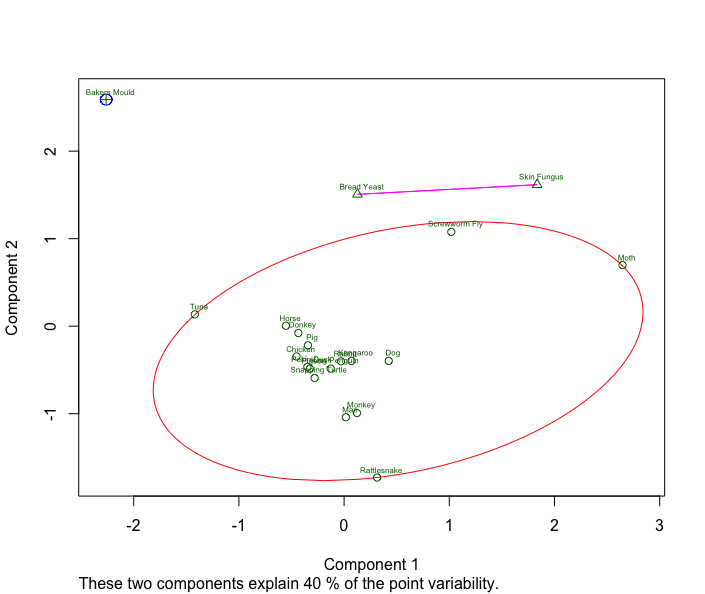
\includegraphics[width=1\linewidth]{img/3-3-mut-K-means-class-1}
		\caption{\small Classification n° 1}
		\label{fig:3-3-mut-K-means-class-1}
	\end{subfigure}%
	\begin{subfigure}[b]{0.5\linewidth}
		\centering
		\captionsetup{justification=centering}
		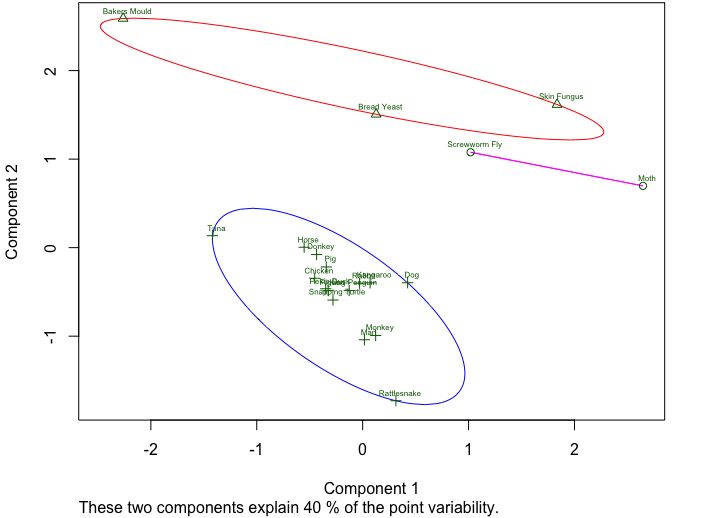
\includegraphics[width=1\linewidth]{img/3-3-mut-K-means-class-2}
		\caption{\small Classification n° 2}
		\label{fig:3-3-mut-K-means-class-2}
	\end{subfigure}%
	\caption{\small Classifications 1 et 2}
\end{figure}
\begin{figure}[H]
	\centering
	\captionsetup{justification=centering, margin=2cm}
	\begin{subfigure}[b]{0.5\linewidth}
		\centering
		\captionsetup{justification=centering}
		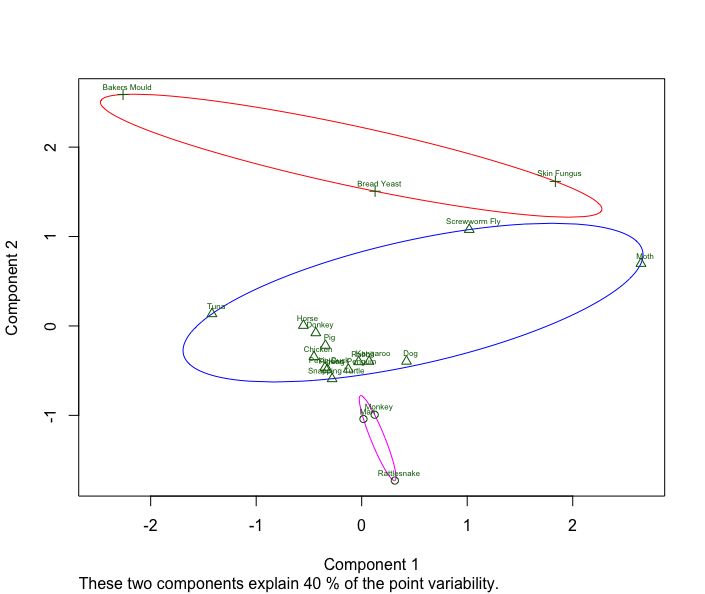
\includegraphics[width=1\linewidth]{img/3-3-mut-K-means-class-3}
		\caption{\small Classification n° 3}
		\label{fig:3-3-mut-K-means-class-3}
	\end{subfigure}%
	\begin{subfigure}[b]{0.5\linewidth}
		\centering
		\captionsetup{justification=centering}
		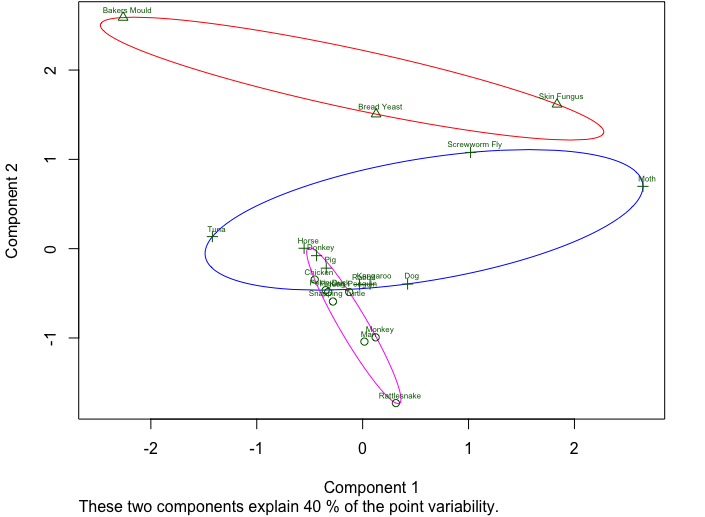
\includegraphics[width=1\linewidth]{img/3-3-mut-K-means-class-4}
		\caption{\small Classification n° 4}
		\label{fig:3-3-mut-K-means-class-4}
	\end{subfigure}%
	\caption{\small Classifications 3 et 4}
\end{figure}
\begin{figure}[H]
	\centering
	\captionsetup{justification=centering, margin=2cm}
	\begin{subfigure}[b]{0.5\linewidth}
		\centering
		\captionsetup{justification=centering}
		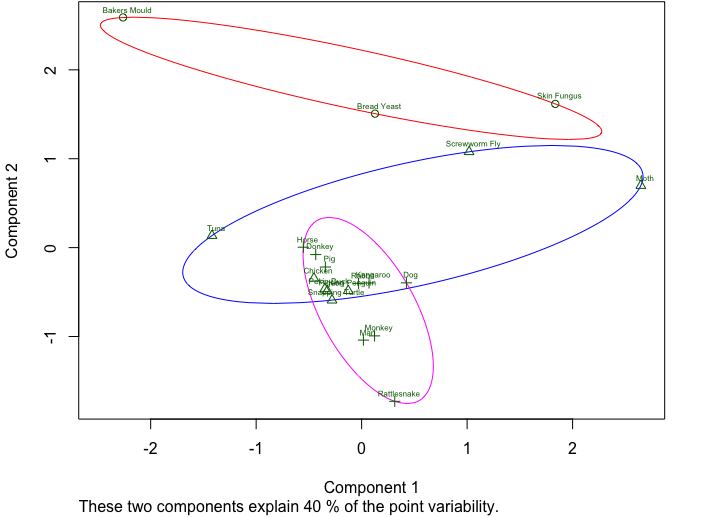
\includegraphics[width=1\linewidth]{img/3-3-mut-K-means-class-5}
		\caption{\small Classification n° 5}
		\label{fig:3-3-mut-K-means-class-5}
	\end{subfigure}%
	\begin{subfigure}[b]{0.5\linewidth}
		\centering
		\captionsetup{justification=centering}
		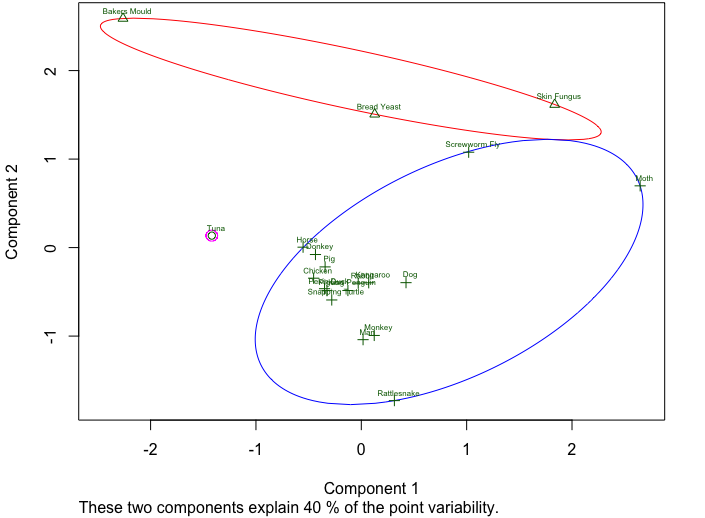
\includegraphics[width=1\linewidth]{img/3-3-mut-K-means-class-6}
		\caption{\small Classification n° 6}
		\label{fig:3-3-mut-K-means-class-6}
	\end{subfigure}%
	\caption{\small Classifications 5 et 6}
\end{figure}


Lorsqu'on observe les représentations graphiques de ces classifications, on remarque plusieurs choses~:
\begin{itemize}
	\item La classification n°1 fait graphiquement sens et rejoint les résultats de la classification hiérarchique (voir \autoref{section:mut-class-hierarchique})~;
	\item La classification numéro 2 fait elle aussi sens : en regroupe certains des individus les plus éloignés et on recentre la classe des éléments proches les uns des autres~;
	\item La classification n°3, bien que d'inertie intra-classe plus importante que la n°2, apparaît plus souvent. Cette classification pourrait faire sens avec notre connaissance préalable des données~: regrouper \textit{Man} et \textit{Monkey} est logique. Notons tout de même qu'il y a aussi le \textit{Rattlesnake} avec, ce qui fait moins sens~;
	\item Les autres classifications sont visiblement mauvaises~: chevauchements de classes, et singleton n'ayant graphiquement pas lieu d'être.
\end{itemize}

\end{document}